%%%%%%%%%%%%%%%%%%%%%%%%%%%%%%%%%%%%%%%%%%%%%%%%%%%%%%%%%%%%%%%%%%%%%
%%%
%%% Set these variables appropriately
%%%
\newcommand{\AUTHORS}{YOUR NAME HERE}
\newcommand{\TITLE}{PAPER TITLE HERE}
\newcommand{\KEYWORDS}{}
\newcommand{\CONFERENCE}{}
\newcommand{\PAGENUMBERS}{yes}       % "yes" or "no"
\newcommand{\TOAPPEAR}{no}
%%%
%%%
%%%%%%%%%%%%%%%%%%%%%%%%%%%%%%%%%%%%%%%%%%%%%%%%%%%%%%%%%%%%%%%%%%%%%

%%%% Setup the document/page
\documentclass[pdftex,twoside,twocolumn,10pt,letterpaper]{article}
\usepackage{ifthen}

\ifthenelse{\equal{\PAGENUMBERS}{yes}}{%
\usepackage[nohead,
            left=1in,right=1in,top=1in,
            footskip=0.5in,bottom=0.75in     % Room for page numbers
            ]{geometry}
}{%
\usepackage[noheadfoot,columnsep=0.2in,
            margin=1in,centering,truedimen]{geometry}
}

\usepackage{fancyhdr}
\usepackage[numbers,sort]{natbib}
\usepackage{xspace}
\usepackage{booktabs}
\usepackage{subfigure}
\usepackage[T1]{fontenc}
\usepackage{textcomp}
\usepackage{mathptmx}   % Times + Times-like math symbols
\usepackage{courier}
\usepackage[scaled=0.92]{helvet}

\usepackage{color}
\usepackage[pdftex]{graphicx}
\ifthenelse{\isundefined{\wantBW}}{%
  \usepackage[colorlinks]{hyperref}%        % for online version
}{%
  \usepackage[pdfborder={0 0 0}]{hyperref}% % for paper (B&W) version
}
\newcommand{\URL}[1]{\url{#1}}

%%%%% Setup for PDF
\hypersetup{%
pdfauthor = {\AUTHORS},
pdftitle = {\TITLE},
pdfsubject = {\CONFERENCE},
pdfkeywords = {\KEYWORDS},
bookmarksopen = {true}
}

%\setlength{\parindent}{0pt}
%\setlength{\parskip}{0pt}
\renewcommand{\headrulewidth}{0pt}
\newcommand{\Paragraph}[1]{\vspace{-2ex}\paragraph{#1.}}
\setlength{\topmargin}{-.15in}

\ifthenelse{\equal{\PAGENUMBERS}{yes}}{%
  \pagestyle{plain}
}{%
  \pagestyle{empty}
}

\makeatletter\long\def\@makecaption#1#2{
   \vskip 10pt
   \setbox\@tempboxa\hbox{\textsf{#1: #2}}
   \ifdim \wd\@tempboxa >\hsize % IF longer than one line:
       \textsf{#1: #2}\par      % THEN set as ordinary paragraph.
     \else                      % ELSE  center.
       \hbox to\hsize{\hfil\box\@tempboxa\hfil}
   \fi}
\makeatother

\clubpenalty=10000  % Don't allow orphans
\widowpenalty=10000 % Don't allow widows

\title{\textbf{\TITLE}}
\author{\AUTHORS}
\date{}

% Compact itemize and enumerate.  Note that they use the same counters and
% symbols as the usual itemize and enumerate environments.
\def\compactify{\itemsep=0pt \topsep=0pt \partopsep=0pt \parsep=0pt}
\let\latexusecounter=\usecounter
\newenvironment{CompactItemize}
  {\def\usecounter{\compactify\latexusecounter}
   \begin{itemize}}
  {\end{itemize}\let\usecounter=\latexusecounter}
\newenvironment{CompactEnumerate}
  {\def\usecounter{\compactify\latexusecounter}
   \begin{enumerate}}
  {\end{enumerate}\let\usecounter=\latexusecounter}

\newcommand{\comment}[1]{\textcolor{red}{#1}}
\newcommand{\ignore}[1]{}

\newcommand{\xc}[1]{\mbox{\textit{#1}}}
\newcommand{\la}{\leftarrow}
\newcommand{\ra}{\rightarrow}
\newcommand{\somespace}{\hspace{0.1cm}}

\def\discretionaryslash{\discretionary{/}{}{/}}
\def\discretionarydot{\discretionary{.}{}{.}}
\def\discretionarycolon{\discretionary{:}{}{:}}
{\catcode`\/\active
\catcode`\.\active
\catcode`\:\active
\gdef\URLprepare{\catcode`\/\active\let/\discretionaryslash
                 \catcode`\.\active\let.\discretionarydot
                 \catcode`\:\active\let:\discretionarycolon
        \def~{\char`\~}}}%
\def\URL{\bgroup\URLprepare\realURL}%
\def\realURL#1{\tt #1\egroup}%

\newcommand{\eg}{{\em e.g.}, }
\newcommand{\ie}{{\em i.e.}, }
\newcommand{\etal}{{\em et al.\ }}

\def\check{\stackrel{{\scriptscriptstyle ?}}{=}}

\begin{document}
\maketitle

% -*-LaTeX-*-
% $Id: abstract.tex 70 2007-01-30 21:59:16Z nicolosi $

\begin{abstract}
Chain replication storage systems such as CRAQ\cite{terrace2009object} target at improving read throughputs for read-mostly workloads. However, write requests can only be handled by the head node of the chain, resulting in low write throughputs. Amazon's Dynamo\cite{decandia2007dynamo} sacrifices strong consistency for high availability, but only eventual consistency is achieved. Neither of these two systems finds the balance point between availability and consistency. From user's point of view, data objects are generally classified as critical and non-critical. Critical objects prefer strong consistency and low write throughput is acceptable, while eventual consistency is sufficient for non-critical objects, but high availability is preferred. Based on this observation, we propose CRAQamo, a storage system which supports strong consistency and eventual consistency at the same time. 
\end{abstract}

   
\section{Introduction}
\label{sec:intro}

Many commercially deployed systems, such as Amazon Dynamo\cite{decandia2007dynamo}, sacrifices strong consistency properties for high availability and throughput, and low latency. This sacrifice is driven by the need of providing client applications with an ``always-on" experience. For example, a customer needs to manipulate items in the shopping cart without any latency, but it is usually acceptable to the customer if deleted items appear again due to conflicts or failures unless it is the final check-out. Another example may be a user trying to change his profile picture. Strong consistency is not required here because the user usually allows some time for the change to take effect. However, when a user places an order in that shopping cart, strong consistency is preferred. Similarly, when users change their privacy settings, they don't want their privacy to be different if somebody happens to hit a different node.

CRAQ\cite{terrace2009object} is a chain replication storage system which guarantees strong consistency, but it targets read-mostly workloads and cannot provide high write throughput and availability and low latency, as every write request needs to go through the head of the chain, and pass through every node, before returning.  Given inexpensive hardware, one can never guarantee strong consistency, high write throughput, high availability, and low latency at the same time. Based on this assumption, we ask the question: in terms of the performance, can we flexibly switch between CRAQ and Dynamo? Can we design a storage system which still supports $put()$ and $get()$ operations, but accepts one more parameter - $consistency$? $consistency$ is a binary flag indicating whether the operation is strongly consistent or eventually consistent.

We call this such system CRAQamo, implying that it is a hybrid of CRAQ and Dynamo. Specifically, when the client application does not require consistency guarantees, like in a shopping cart, CRAQamo only supports eventual consistency. When the client application requires strong consistency, for example, in the customer's list of orders, CRAQamo sacrifices write latency to guarantee strong consistency. CRAQamo is not a system which simply runs CRAQ and Dynamo in parallel, because each of these two systems have their own arrangements of nodes, failure detection and recovery strategies, and data would be difficult to share between the systems. CRAQamo merges them into a single system for maximal efficiency, and ease of use.


\section{Design}
\label{sec:design}

\subsection{General framework}
In CRAQamo, each read or write request is given a tag of consistency requirement: strong or eventual. Strongly consistent reads and writes are performed as standard CRAQ operations. Enventually consistent read requests can go to any node in the chain like CRAQ, but the most recent data is returned before confirming that every server has updated to that value. Enventually consistent write requests can be served by any node as well, but the written value is send to other servers using ``multicast'' instead of propagating from the head node to the tail node. In practice we define values, $W$ and $R$. Before a server responds to a read request, it must synchronize with the other servers and wait to return until there are at least $R$ successful responses, then reply back to the user.  Before a server responds to a write request, it must synchronize with other servers and wait until there are at least $W$ successful responses. Effectively we implemented a system where a certain number of participants must agree on a value before it can be committed. With both strongly and eventually consistent operations supported in CRAQamo we can meet the the users' consistency and performance requirements in different application scenarios using a single infrastructure. 

Intuitively, lowering the consistency constraint to eventual consistency can help us achieve much better write latency and throughput, however, the read performance may degrade slightly due do pair-wise communications between servers to compare data versions. The improvements and overheads will be presented quantitatively in our evaluations. The performance advantage of eventual consistenty becomes more obvious as we increase the communication latency between servers to simulate data centers that spread around the globe. We modified the CRAQ source code and implemented data propagation and synchronization procedures using the same RPC interface as CRAQ. The network latency is controlled by port forwarding using ``ncat" program which is able to redirect data from one network port to another while adding a controlled amount of latency.

\subsection{Original CRAQ capabilities}
Our system is built upon CRAQ, thus it has the full capabilities of CRAQ. CRAQ naturally supports strongly consistent read and write. We keep the strongly consistent storage interfaces in CRAQ and leave an additional flag for the user to determine whether to apply strongly consistent operations. We also adopt the failure recovery mechanism in CRAQ.

\subsection{Internal methods}
{\noindent \bf Broadcasting data\ \ }In CRAQ, data is only passed between neighboring nodes, which causes the write operations to be inefficient because each write operation needs to go through all the nodes although strong consistency is guaranteed. In CRAQamo, when strong consistency is not a must, we allow direct communication between any two nodes. Specifically, we have an internal method called ``eventual consistency propagate'' to help pass information globally among all the nodes. We show the necessity of having this internal helper method in the following sections. \\

{\noindent \bf Comparing versions\ \ }Like CRAQ, each node in the chain also store multiple versions of objects in CRAQamo. CRAQ uses a monotonically-increasing number as the version number, which is local to the node. Synchronization is not a problem to CRAQ since as we mentioned previously, data is only passed between neighboring nodes. However, such a simple representation for the version cannot handle global broadcasting and race conditions well. Instead, CRAQamo uses global timestamps to represent versions. We would like to emphasize that replacing monotonically-increasing version numbers with timestamps do not affect the original functionalities of CRAQ, thus strongly consistent operations are still supported by CRAQ and we do not discuss them in detail here.

For eventually consistent operations, we need to remotely compare versions of objects between nodes. Therefore it is necessary for each node to fetch the newest timestamps on other nodes and determine if either node needs to be updated. Specifically, a node signals other nodes to return their current timestamps. Since the timestamps are global, comparison and be easily done by comparing the actual values of timestamps (larger value means newer and vice versa). Such version comparing method also serves as an internal helper method and we detail the usages in the following sections. 

\subsection{Eventually consistent read}
Eventual consistency allows read operations to return newly written objects before they are fully synchronized among all nodes. This is the key to reducing the read latency comparing with CRAQ because CRAQ is constrained by the strong consistency capability, thus only committed objects can be returned. In the eventual consistency mode of CRAQamo, the newly written object can be directly returned to the requester as long as the timestamp of the object is sufficiently new. Note that it is not strictly required that the timestamp of the object on the current node is the newest. We apply a Dynamo style parameter $R$ so that the user can determine the level of eventual consistency.

When an eventually consistent read operation is performed on a node. The node first compares the timestamp of the requested object with the timestamps of the object on all other nodes. To speed up the process, the comparisons are done in parallel. Once $R$ other nodes agree that the current node has the newer version of object, the current node directly returns the object to the user. If any of the $R$ nodes disagree that the current node has the newest version of object, the requesting node updates itself to the most recent version. If any of the other nodes are not up to date, the requesting node sends an ``eventual consistency propagate" request to that node.  By varying $R$, the level of eventual consistency can be flexibly tuned. For example, lowering $R$ requires fewer nodes to be synchronized before returning to the client so that the overall read latency can be reduced.

\subsection{Eventually consistent write}
A critical reason that chain replication storage systems are generally slow in write operations is that the write operation needs to go through all the nodes in the chain. While this guarantees strong consistency, the latency is also large when latency between nodes is large. However, if strong consistency is not a must, one can choose to write new data to any node in the chain instead of writing to the head node. In CRAQamo, we allow the user to write to any node and safely check whether there are other writes performed on other nodes when the write operation is being performed. Note that write operations happening almost concurrently on multiple nodes rarely happens, so the synchronization can take slightly longer time and it will not critically affect the overall write performance.

When an eventually consistent write operation is performed on a node. The node first takes the input object, writes it locally and attaches a timestamp to the updated object. It then calls ``eventual consistency propagate" to broadcast that new value to the other nodes.  When the other nodes receive that propagation, they confirm the sent version is the latest.  If it is, they write the value and return, but if it isn't, they propagate their value to the node that sent the original propagate.  After the original node agrees on the new value and returns from the propagate, the target node returns successfully. Once the original node has reached a consensus with $W$ other nodes, it returns a success to the client, and continues the propagation algorithm with the remaining nodes. 

\subsection{Implementation}
Our prototype implementation of CRAQamo was implemented in approximately 3700 lines of C++,
built upon the a prototype implementation of CRAQ implemented in approximately 3000 lines of C++.
Like CRAQ, CRAQamo uses the Tame \cite{tame} extension to the SFS asynchronous I/O and RPC libraries \cite{sfs} and all network functionality between CRAQamo RPC nodes is exposed via Sun RPC interfaces.
Unlike CRAQ, CRAQamo also uses the built in C++ multithreading library.
To implement the broadcast reads and writes for consistency checks, CRAQamo needs to spin up multiple threads, and wait until $w$ of them complete their calls before returning.
Even after returning, however, CRAQamo needs to continue the consistency checks for the nodes that have not completed.
This proved too difficult of a pattern to express in Tame, so we instead built our own manner of multithreading for these checks.
However, for all other asynchronous calls, we used Tame to decrease code complexity.

Our integration with ZooKeeper was provided with by the expansion of CRAQ, and was integrated in the same way, with CRAQamo nodes able to query the same ZooKeeper files as CRAQ nodes.
Furthermore, expansion of CRAQ gave us free chain node functionality and the ability to handle membership changes dynamically.
Because data is stored in the same manner as CRAQ, and because no node has special knowledge in CRAQamo, CRAQ's algorithm for membership changes proves sufficient for CRAQamo.

\section{Evaluation}
\label{sec:eval}

\subsection{Experiment setups}
We deployed ZooKeeper service and the CRAQamo server nodes on Princeton University's $tux.cs.princeton.edu$ virtual machines.
These machines have 4 Intel(R) Xeon(R) CPUs which each run at 3.07GHz. The nodes were configured to listen on local network ports for our testing to be both easier and more consistent. To simulate the high communication latency that might occur when servers are geopraphically separated or operating under bad network environment, we used ``ncat'' in port forwarding mode to receive request connections on a different network port, then relay the data with a controlled delay to the actual listening port of CRAQamo servers. The delay is inserted in a per data line fashion which differs from the per-packet latency that exists in real TCP/IP networks. In our setting the amount of delay in $x$ miliseconds will
translate to $2x$ milisecond of round trip time, or RTT in real long range network communications. 

We used a chain size of 3 nodes for the tests, and the eventually consistent requests are replied when 2 servers respond (including the one handling the request). A client program that generates requests at a fixed rate is used to test the latency of CRAQamo's operations. For our latency tests, we sent the server read and write requests at a rate much underneath the servers' throughput threshold, and calculated the time from request to response.  To generate the desired proportions of operations, we ran multiple clients sending requests at a configurable number of requests per second.  For our throughput tests, we sent the server read and write requests at a rate higher than the throughput, and saw how many it was able to respond to in $5$ seconds.

\subsection{Effects of network delay on latency}
\begin{figure}[hbt]
\centering
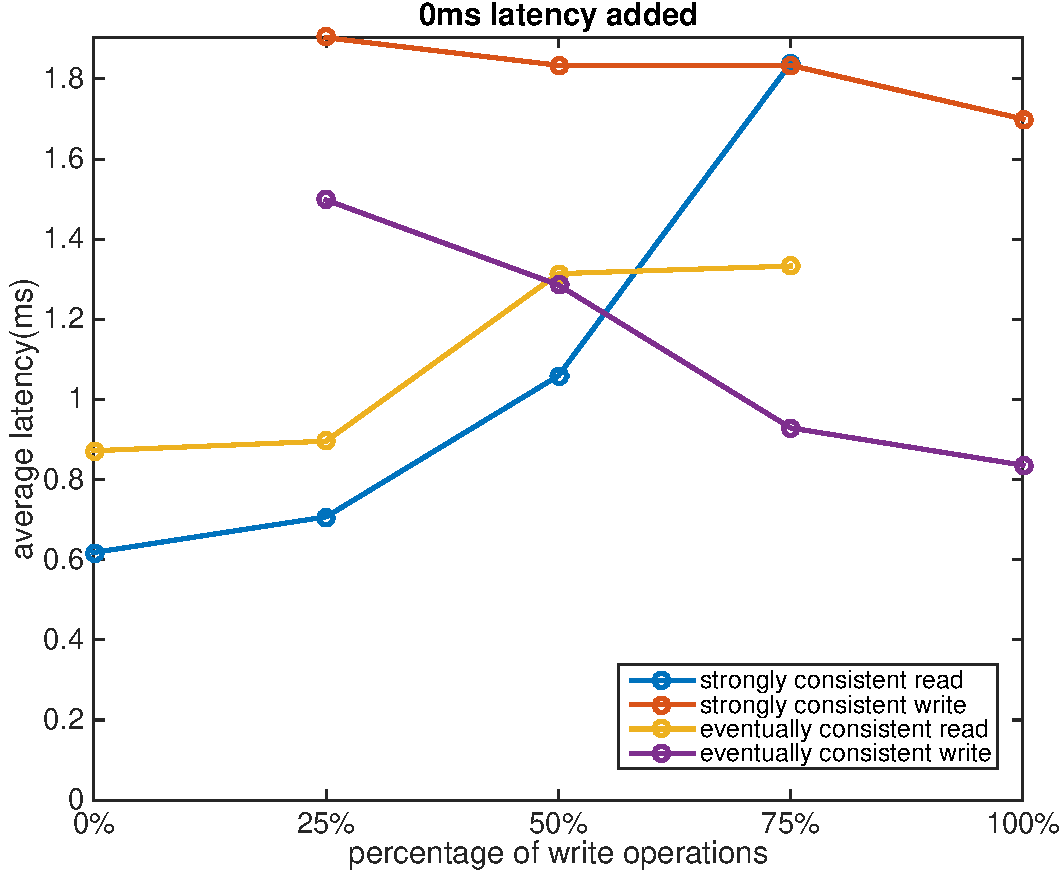
\includegraphics[width=\linewidth]{figures/latency_0.pdf}
\caption{with no network delay}
\label{fig:latency_0}
\end{figure}

\begin{figure}[hbt]
\centering
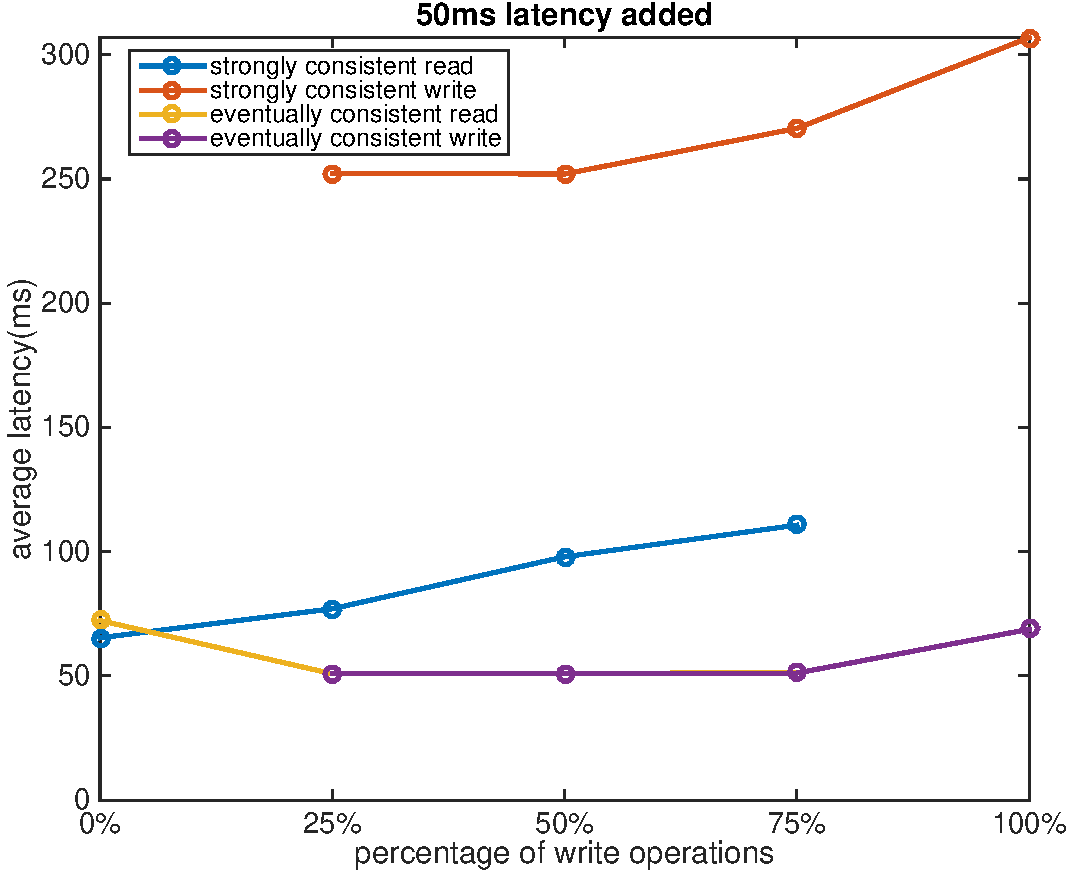
\includegraphics[width=\linewidth]{figures/latency_50.pdf}
\caption{with 50ms network delay}
\label{fig:latency_50}
\end{figure}

\begin{figure}[hbt]
\centering
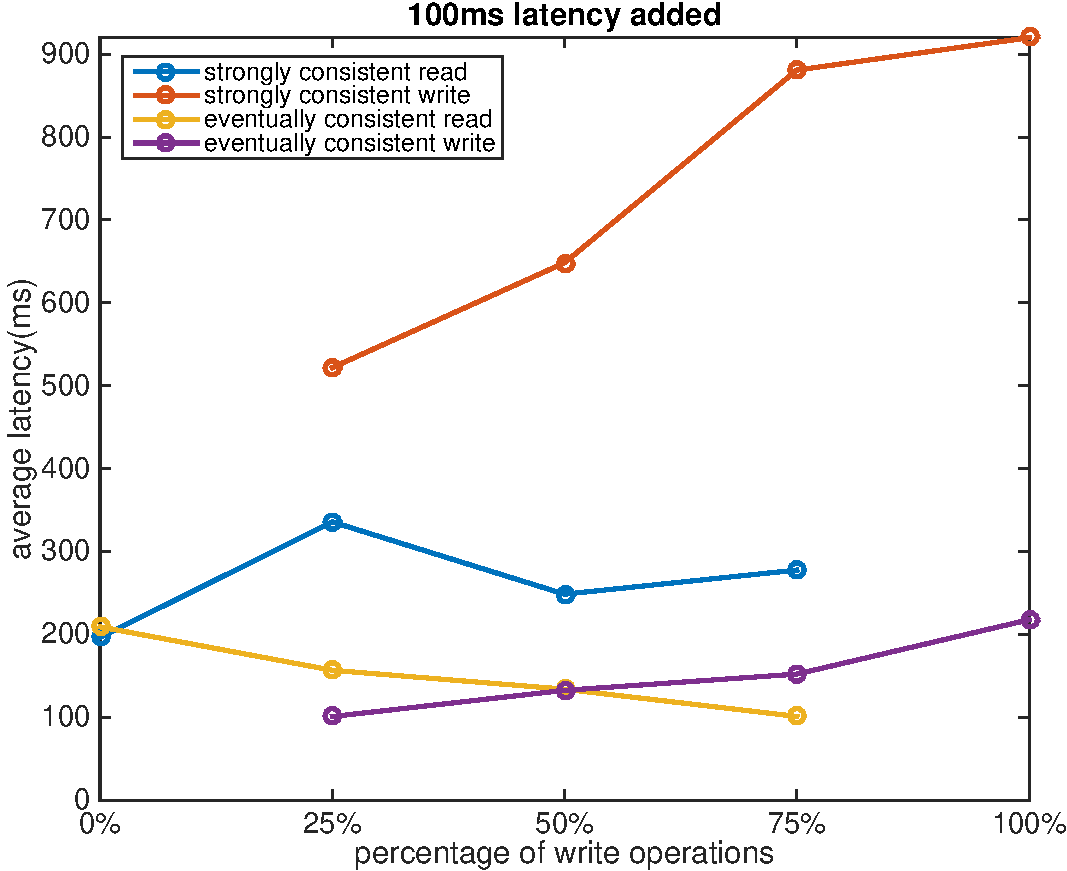
\includegraphics[width=\linewidth]{figures/latency_100.pdf}
\caption{with 100ms network delay}
\label{fig:latency_100}
\end{figure}
\vspace{-2mm}


CRAQamo was tested using 3 different network delay amounts of 0ms, 50ms and 100ms. We also varied the proportion of write requests to better illustrate CRAQamo's ability to support faster writes in eventual consistency model. We recorded the average latency of the four types of requests, namely strongly consistent read (SC read), strongly consistent write (SC write), eventually consistent read (EC read), and eventually consistent write (EC write). SC operations are the ones supported by the original CRAQ. Note that SC and EC operations are not mixed togather for this section of evaluation, therefore SC reads are only executed together with SC writes while EC reads are only executed together with EC writes. 

Under perfect network conditions , EC reads are slightly slower than SC reads when write operations are not dominant (see Figure \ref{fig:latency_0}), because EC reads needs multiple servers to agree on a value before replying back to the client while in most cases in SC mode, the servers know that their copy of the data is the most recent committed, this is one of CRAQ's selling point. As there are more writes SC reads get slower than EC read because writes must propagate in the chain. EC writes are consistently faster than SC writes under different write proportions due to the fact that EC writes does not need to go from chain head to chain tail sequencially.

With 50ms of network delay (100ms RTT), latency of EC operations differentiate from SC operations  (see Figure \ref{fig:latency_50}). EC reads can take almost 50\% less time than SC reads when there are more write requests, while EC writes are close to 5 times faster than SC writes on average. The gain comes from sacrificing consistency.

When network delay is more significant at 100ms (200ms RTT), typical for a long distance network connection, EC operations really show their advantage in latency  (see Figure \ref{fig:latency_100}). Latency of EC reads and writes stay in the range of 100ms to 200ms, for different write proportions, while SC operations become intolerably irresponsive (e.g., SC write at almost 900ms with 75\% writes).

\subsection{Effect of mixing different consistency models}
\vspace{-2mm}
\begin{figure}[hbt]
\centering
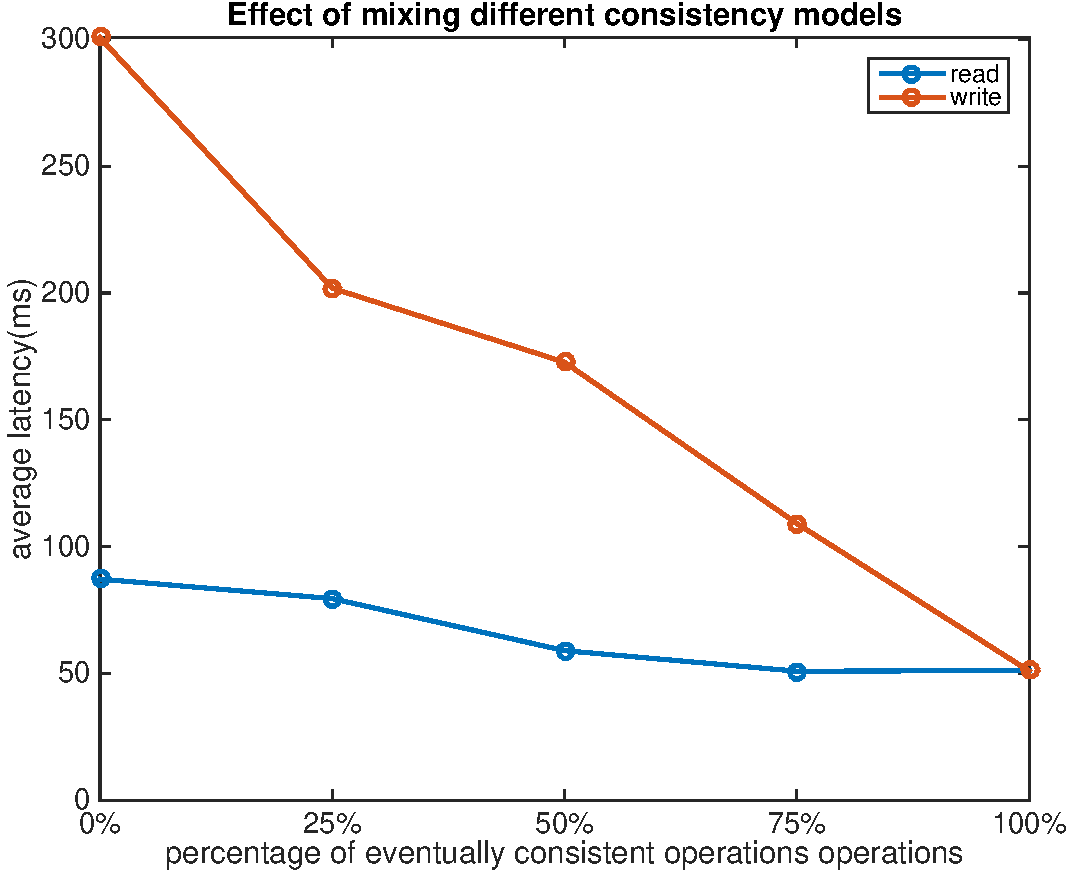
\includegraphics[width=\linewidth]{figures/mix.pdf}
\caption{mixing SC/EC operations - average latency}
\label{fig:mix}
\end{figure}
\vspace{-5mm}

\begin{figure}[hbt]
\centering
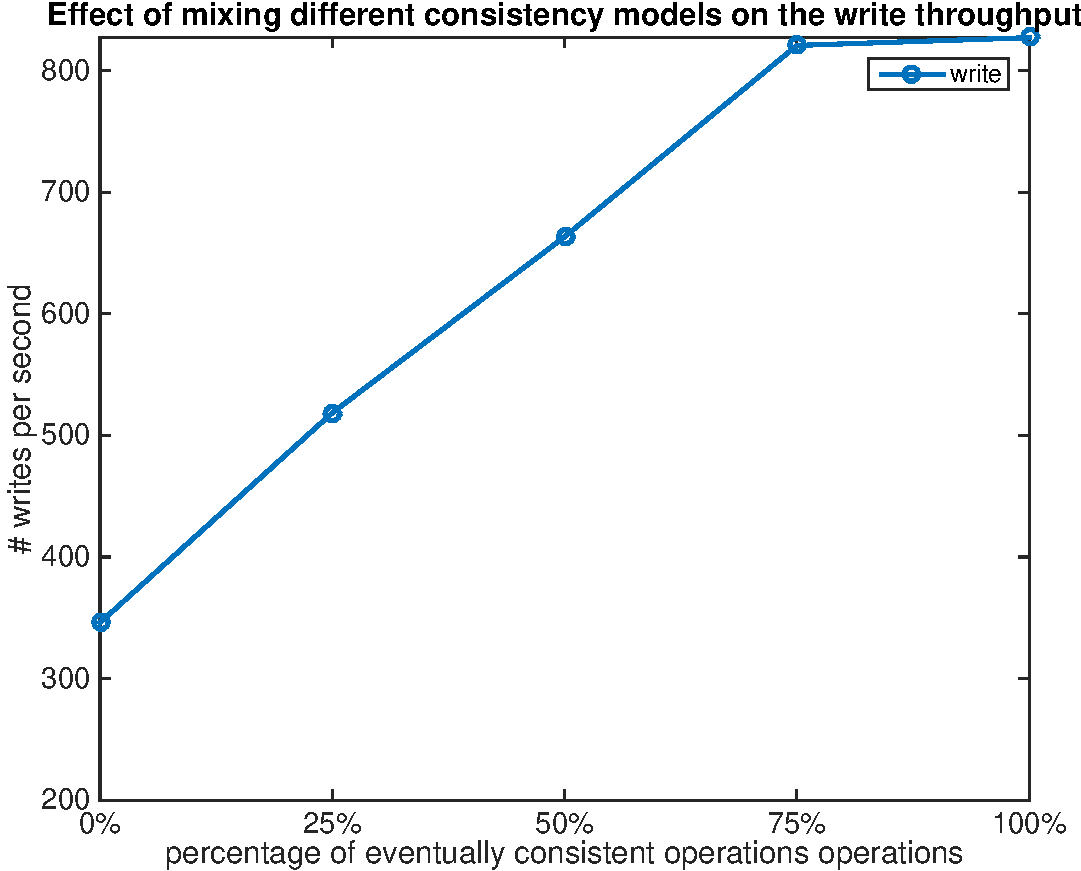
\includegraphics[width=\linewidth]{figures/throughput.pdf}
\caption{mixing SC/EC operations - write throughput}
\label{fig:mix_throughput}
\end{figure}


To analyse the effect on latency of mixing SC/EC operations, we tested CRAQamo with varying proportions of EC/SC operations at 50\% writes and 50ms delay using the same setup from the previous section. The average latency of read and write operations (including both SC and EC) is shown in Figure \ref{fig:mix} and the write throughput is shown in Figure \ref{fig:mix_throughput}.  As there are more EC operations inflight, the average latency dropped fast monotonically and the write throughput improves significantly. Indeed EC operations can be executed much faster and are suitable for non-critical data. 



\section{Related Work}

%\subsection{Chain Replication (CR)}
{\noindent \bf Chain Replication (CR)\ \ } The chain replication (CR) storage system is a distributed object storage system which is capable of providing strongly consistent operations. In chain replication, data-centers (or nodes) are linked in a chain in which only neighboring communication is allowed in normal cases. In CR, All read operations are handled by the tail and all write operations are handled by the head. During writing, the new data needs to be propagated from the head to the tail until the updated object is marked as committed. When a read request occurs, the tail node simply returns the newest committed object. While the working mechanism of CR is simple, it is obvious that the latency of both read and write operations can be very high, especially when the nodes are placed geographically distant to each other. The situation gets even worse for write operations because the new data needs to be propagated all the way from the head to the tail and it also results in high latency. \\

%\subsection{CRAQ}
{\noindent \bf CRAQ\ \ } CRAQ\cite{terrace2009object} is a variant of the chain replication storage system and it targets at improving the throughput of strongly consistent read operations by allowing users to access data from any node in the chain. The idea is to let each node keep multiple versions of data, and to use a flag indicating whether the version is {\it dirty} or {\it clean}. {\it Clean} flag means that the version is committed and it is safe to directly return it to the requester. {\it Dirty} flag means that the newly written data has not been committed. Then the current node needs to ask the tail for the latest committed version number and returns the data associated with that version number. This modification greatly improves the read throughput of CR as in most cases, the newest version of object is ready to be returned. CRAQ also naturally supports eventually consistent read operations because each node keeps multiple versions of objects and eventual consistency read can be easily achieved by directly returning the latest version. However, CRAQ only supports strongly consistent write operations, so the write latency still remains a bottleneck for CRAQ. \\

%\subsection{Dynamo}
{\noindent \bf Dynamo\ \ } Dynamo\cite{decandia2007dynamo} is a high available key-value storage system deployed by Amazon. The main observation through Amazon's own services is that sometimes availability and efficiency is highly preferred so that it is possible to sacrifice strong consistency for high availability and efficiency. In order to further increase write throughput, conflict resolution is executed during read instead of write so that write operations look instant to the clients, giving an "always-on" experience. One major advantage of Dynamo is allowing users to tune a few parameters including the number of replicas, the number of read confirmations and the number of write confirmations so that the trade-offs are always in control. For example, increasing the number of write confirmations, although increases consistency, increases the latency at the same time. In CRAQamo, we adopt the parameter tuning idea in Dynamo to control the consistency. \\

%\subsection{Eiger}
{\noindent \bf Eiger\ \ } Eiger\cite{lloyd2013stronger} is a geo-replicated storage system which provides low latency, causal consistency, read-only and write-only transactions. All client requests can be satisfied in the local data center. Eiger supports useful data model abstractions such as column-families and counter columns which provides rich structure allowing programmers to represent and query data efficiently. Eiger provides causal consistency and allows clients to access data with non-blocking read-only and write-only transactions. The problem of Eiger is that all the objects applies a single consistency model. In practice, some objects require strong consistency while others do not, and causal consistency doesn't fix this problem. 
\label{sec:related}


\section{Conclusions}
%\vspace{-3mm}
This paper presents the design and implementation of CRAQamo, a storage system built upon CRAQ, but is capable of mixing different consistency models. Moreover, the level of consistency can be tuned by the user in a Dynamo style. The key observation and motivation of CRAQamo is that not all operations are necessary to be strongly consistent, thus it is sometimes reasonable to adopt eventually consistency for non-critical operations. We demonstrate through experiments that CRAQamo can significantly reduce the latency, and increase the throughput, of CRAQ because of the constraint of strong consistency. We believe that real applications based on object storage systems can benefit from CRAQamo because of the flexibility of choosing consistency and the overall latency can be minimized to the largest extent.
\label{sec:conclusion}



%% Bibliography
%\vspace{-1ex}
%\linespread{1.0}
%\setlength{\bibsep}{1pt}
%\footnotesize
\small
\bibliography{ref}
\bibliographystyle{abbrvnat}

\end{document}

